\subsection{GENERADOR ALEATORIO DE PDU}
%*********************
\begin{frame}{}

\pgfdeclareimage[width=\paperwidth,height=\paperheight]{bg}{imagenes/fondo_lab}
\setbeamertemplate{background}{\pgfuseimage{bg}}

\bfseries{\textrm{\LARGE Lab17\\ \Large GENERADOR ALEATORIO DE PDU}}
\raggedright
\end{frame}
%*********************




%\end{frame}
%---------------------------------

\begin{frame}{PASO 1: UNIDADES DE DATOS DE PROTOCOLOS (PDU)}

\begin{figure}[H]
\centering
\vspace{-3mm}
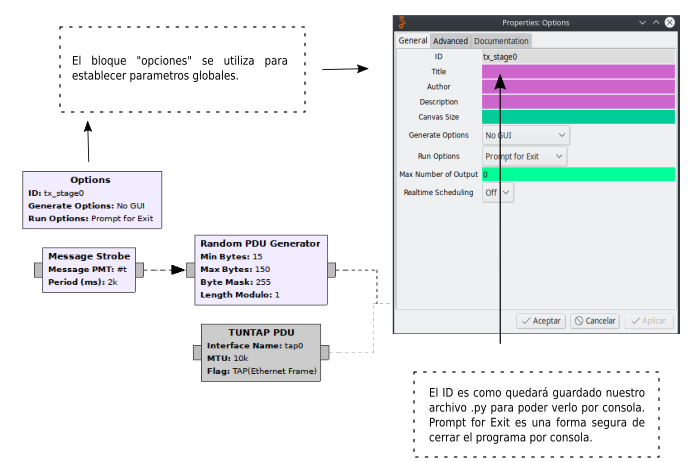
\includegraphics[width=\textwidth]{Modulaciones_digitales/lab25/pdf/primera1.pdf}
\end{figure}

\end{frame}
%---------------------------------

\begin{frame}{PASO 1: UNIDADES DE DATOS DE PROTOCOLOS (PDU)}

\begin{figure}[H]
\centering
\vspace{-3mm}
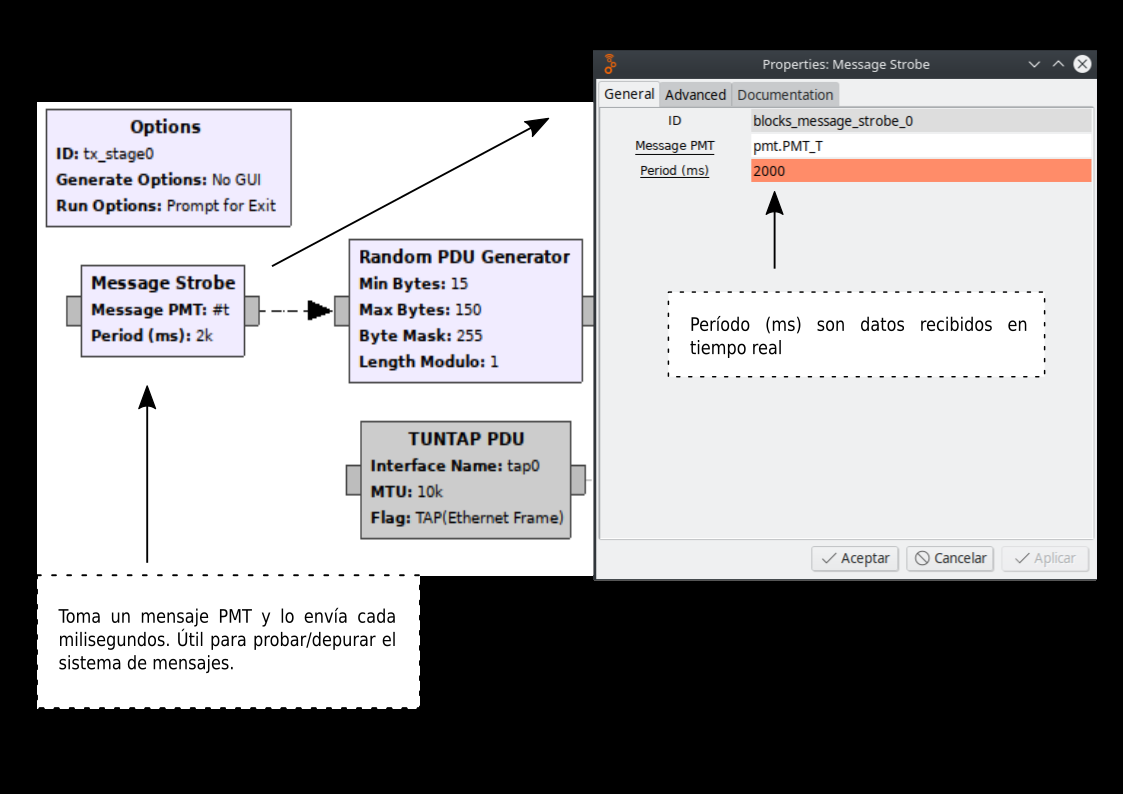
\includegraphics[width=\textwidth]{Modulaciones_digitales/lab25/pdf/bitmap2.pdf}
\end{figure}

\end{frame}
%---------------------------------

\begin{frame}{PASO 1: UNIDADES DE DATOS DE PROTOCOLOS (PDU)}

\begin{figure}[H]
\centering
\vspace{-3mm}
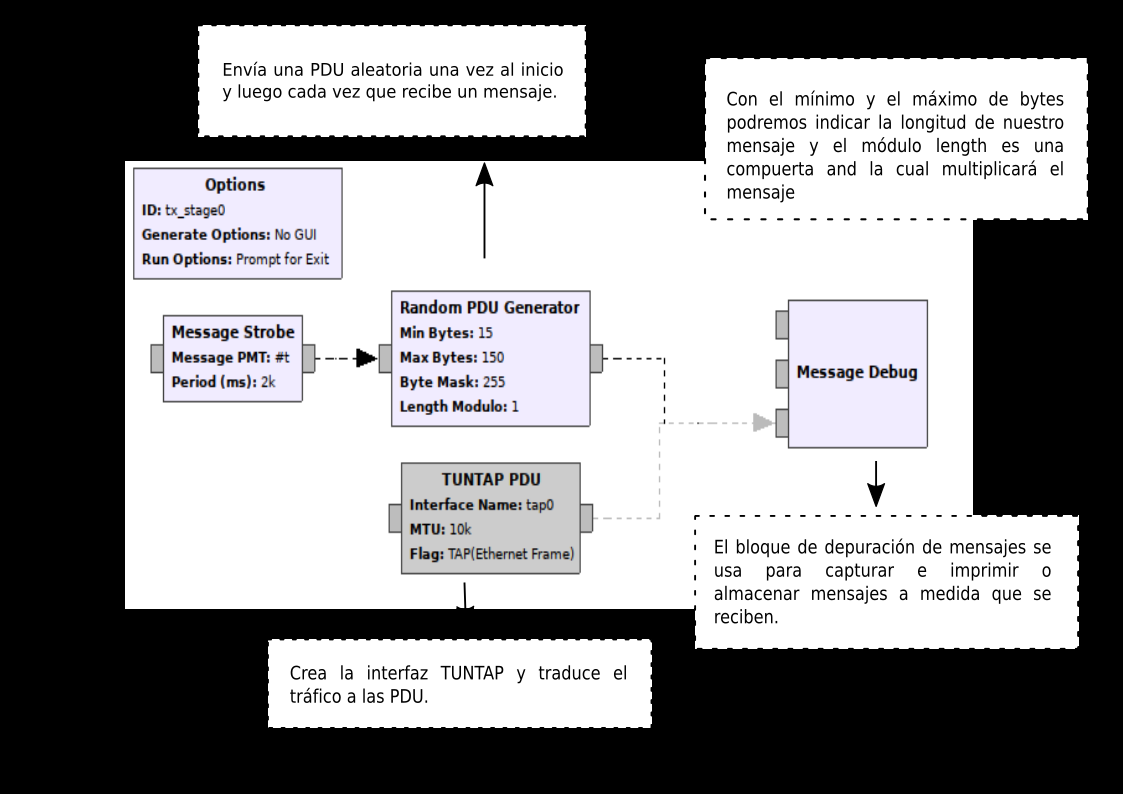
\includegraphics[width=\textwidth]{Modulaciones_digitales/lab25/pdf/bitmap3.pdf}
\end{figure}

\end{frame}
%---------------------------------

\begin{frame}{PASO 1: UNIDADES DE DATOS DE PROTOCOLOS (PDU)}

\begin{figure}[H]
\centering
\vspace{-3mm}
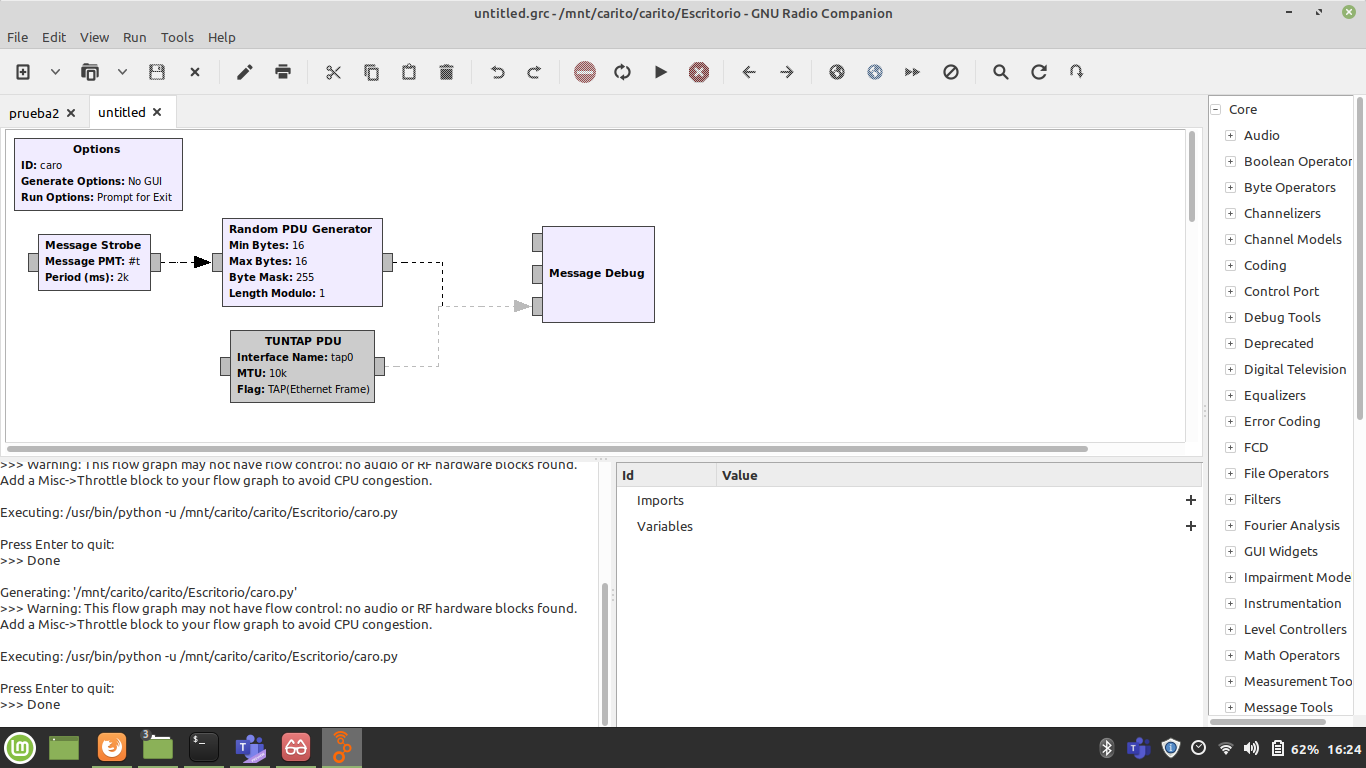
\includegraphics[width=\textwidth]{Modulaciones_digitales/lab25/pdf/panel.pdf}
\end{figure}

\end{frame}
%---------------------------------

\begin{frame}{RESPUESTAS POR MEDIOS DE INTERFAZ GRÁFICA}

\begin{figure}[H]
\centering
\vspace{-3mm}
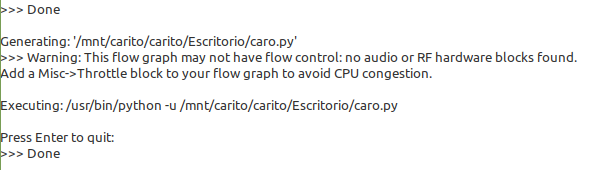
\includegraphics[width=\textwidth]{Modulaciones_digitales/lab25/pdf/mensajespanel.pdf}
\end{figure}

\end{frame}

%---------------------------------



\begin{verbatim}

REPUESTA POR CONSOLA 

  * MESSAGE DEBUG PRINT PDU VERBOSE *
() pdu length = 125
contents =
0000: d0 22 e7 d5 20 f8 e9 38 a1 4e 18 8c 47 30 8c fe
0010: f5 ff f7 f7 28 b9 f8 fb f5 1c 7c cc cc 4c 24 01
0020: 6b 1c ea a3 ca e0 f5 80 a7 cc 09 5c d9 36 ef ae
0030: ad 66 c1 bd be 79 64 6c a7 2c 2b 4d b4 cc 08 51
0040: 46 df 0b 26 18 fe d2 d2 b1 20 51 c3 f3 7d 08 a9
0050: 70 20 61 35 c3 0d cb 09 2f 68 7d 75 72 7c a5 cb
0060: b5 eb c1 ce 46 b4 ae 00 a7 b5 29 a4 1e 74 7f c6
0070: f5 92 57 e0 95 ce 39 04 c0 d2 41 d2 81
***********************************
Press Enter to quit:

\end{verbatim}


%---------------------------------
\begin{frame}{DEFINICIONES}


\begin{description}

    \item[PTM] Los tipos polimórficos se utilizan como portadores de datos de un bloque
/ subproceso a otro.\\ \vspace{2mm}
    \item[PDU]Una PDU (unidad de datos de protocolo) en GNU Radio tiene un tipo
PMT especiales un par de diccionario y un tipo de vector uniforme.\\ \vspace{2mm}

\end{description}
\end{frame}
%---------------------------------

\begin{frame}{PASO 2: DETECCION DE ERRORES CRC}

\begin{figure}[H]
\centering
\vspace{-3mm}
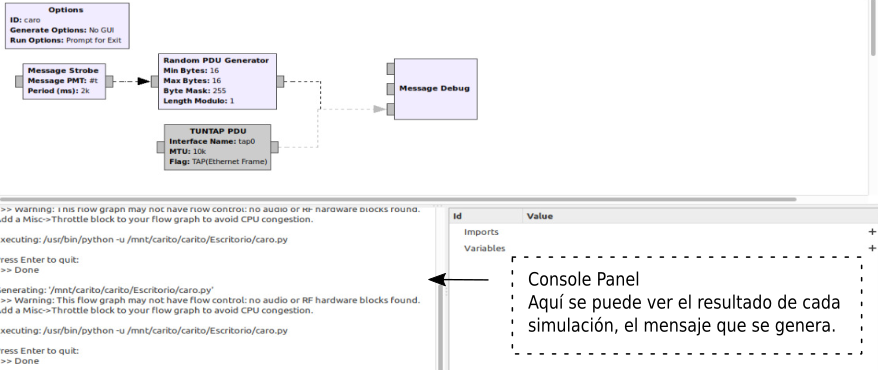
\includegraphics[width=\textwidth]{Modulaciones_digitales/lab25/pdf/cappan.pdf}
\end{figure}

\end{frame}
%---------------------------------

\begin{frame}{ANEXO DE CÓDIGO DE COMPROBACIÓN DE ERRORES (PDU CON CRC)}

\begin{figure}[H]
\centering
\vspace{-3mm}
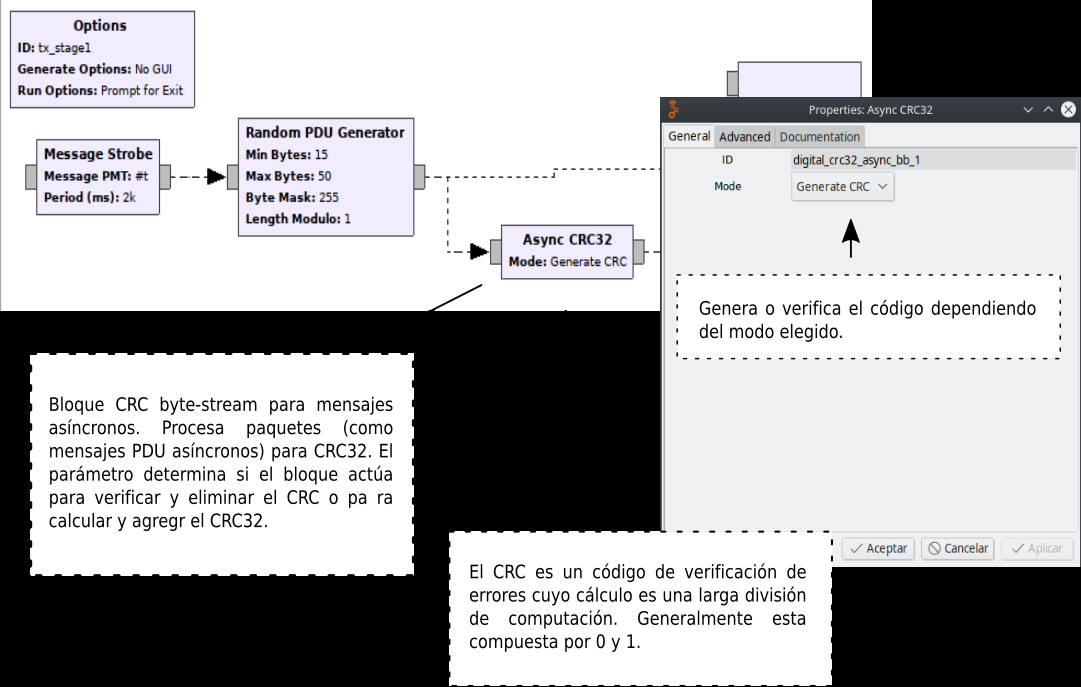
\includegraphics[width=\textwidth]{Modulaciones_digitales/lab25/pdf/bitmap5.pdf}
\end{figure}

\end{frame}
%---------------------------------
\begin{frame}{CALCULADORA DE CRC32}


\begin{description}

    \item[] a mecánica de la informática con su lenguaje binario produce unas
CRC simples. Los bits representados de entrada son alineados en una fila, y el
(n + 1) representa el patrón de bits del divisor CRC (llamado polinomio) se
coloca debajo de la parte izquierda del final de la fila. Aquí está la primera
de ellas para el cálculo de 3 bits de CRC:\\ \vspace{2mm}

\end{description}
\end{frame}
%---------------------------------
\begin{frame}{CALCULADORA DE CRC32}


\begin{figure}[H]
\centering
\vspace{-3mm}
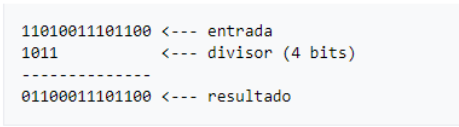
\includegraphics[width=\textwidth]{Modulaciones_digitales/lab25/pdf/calculadora1.pdf}
\end{figure}

\end{frame}
%---------------------------------
\begin{frame}{CALCULADORA DE CRC32}

\begin{description}

    \item[] Si la entrada que está por encima del extremo izquierdo del divisor
es 0, no se hace nada y se pasa el divisor a la derecha de uno en uno. Si la
entrada que está por encima de la izquierda del divisor es 1, el divisor es
(Or) exclusiva en la entrada (en otras palabras, por encima de la entrada de
cada bit el primer bit conmuta con el divisor). El divisor es entonces
desplazado hacia la derecha, y el proceso se repite hasta que el divisor llega
a la derecha, en la parte final de la fila de entrada. Aquí está el último
cálculo.\\ \vspace{2mm}

\end{description}
\end{frame}
%---------------------------------
\begin{frame}{CALCULADORA DE CRC32}


\begin{figure}[H]
\centering
\vspace{-3mm}
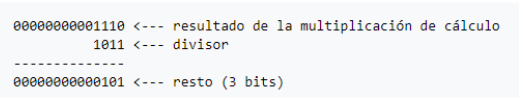
\includegraphics[width=\textwidth]{Modulaciones_digitales/lab25/pdf/calculo2.pdf}
\end{figure}

\end{frame}
%---------------------------------

\begin{frame}{ANEXO DE CÓDIGO DE COMPROBACIÓN DE ERRORES (PDU CON CRC)}

\begin{figure}[H]
\centering
\vspace{-3mm}
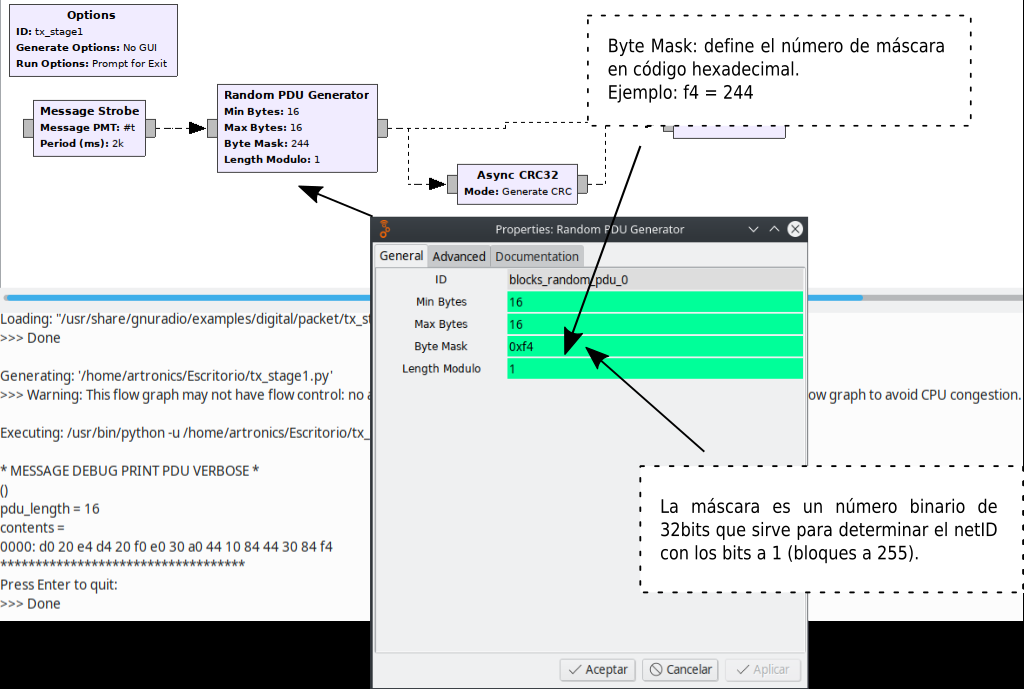
\includegraphics[width=\textwidth]{Modulaciones_digitales/lab25/pdf/bitmap6.pdf}
\end{figure}

\end{frame}
%---------------------------------

\begin{frame}{REPUESTA POR MEDIO DE CONSOLE PANEL}

\begin{figure}[H]
\centering
\vspace{-3mm}
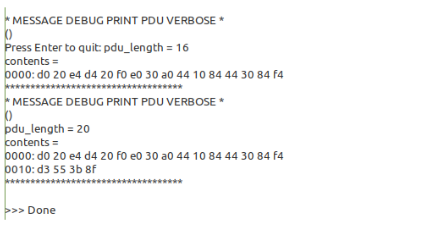
\includegraphics[width=\textwidth]{Modulaciones_digitales/lab25/pdf/f4.pdf}
\end{figure}

\end{frame}
%---------------------------------


\begin{verbatim}

REPUESTA POR CONSOLA 

  * MESSAGE DEBUG PRINT PDU VERBOSE *
() pdu length = 20
contents =
0000: d0 20 e4 d4 20 f0 e0 30 a0 44 10 84 44 30 84 f4
0010: d3 55 3b 8f
***********************************
Press Enter to quit:

\end{verbatim}

%---------------------------------


\begin{frame}{EJEMPLO CON MASCARA PAR}

\begin{figure}[H]
\centering
\vspace{-3mm}
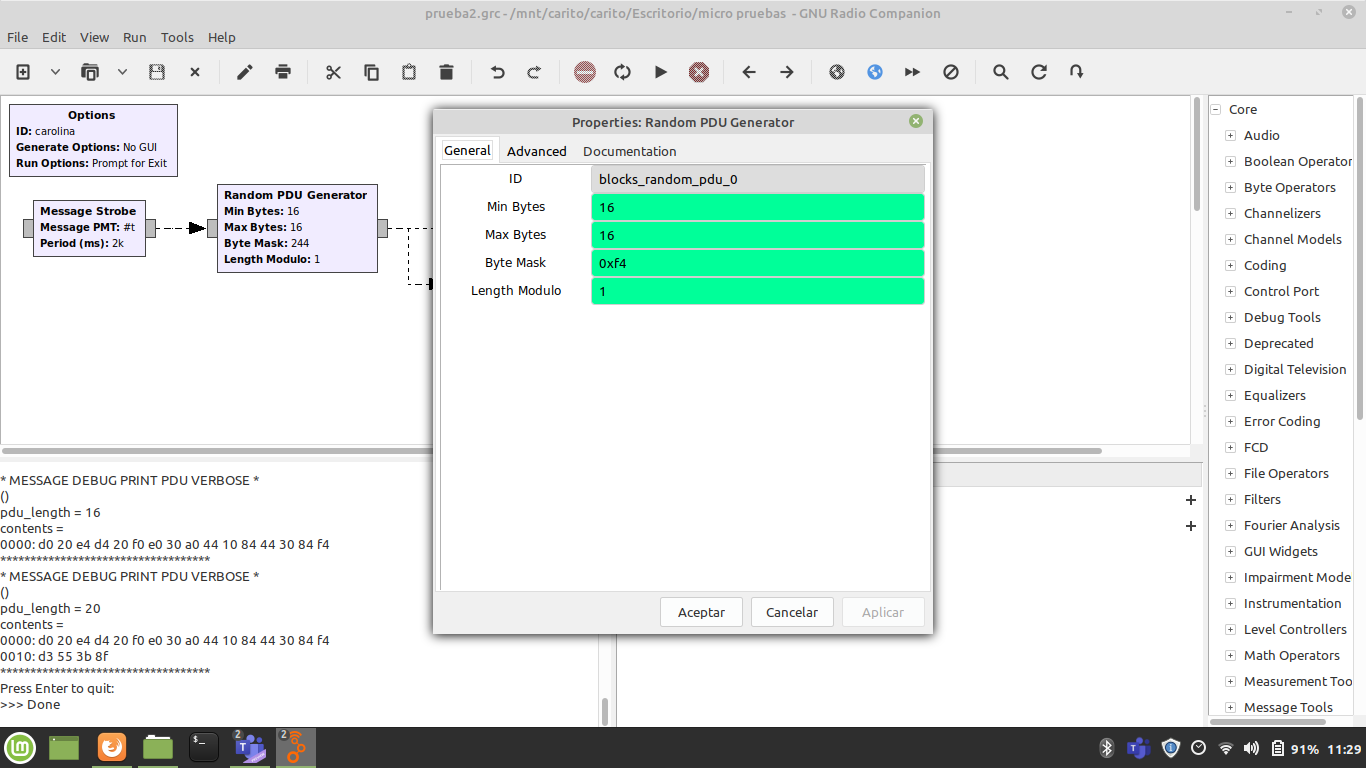
\includegraphics[width=\textwidth]{Modulaciones_digitales/lab25/pdf/maspar.pdf}
\end{figure}

\end{frame}
%---------------------------------

\begin{frame}{CALCULADORA DE CRC32}

\begin{figure}[H]
\centering
\vspace{-3mm}
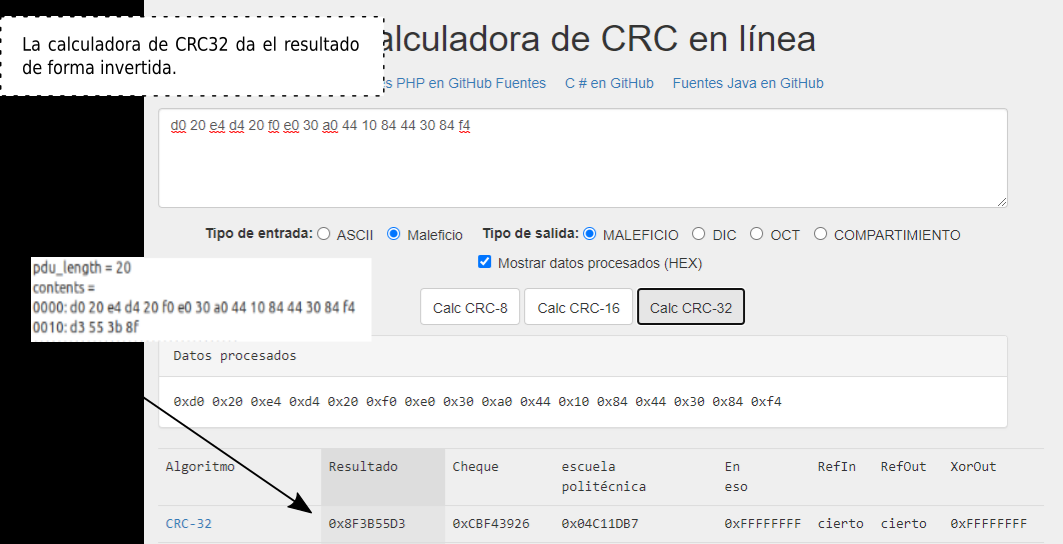
\includegraphics[width=\textwidth]{Modulaciones_digitales/lab25/pdf/bitmap9.pdf}
\end{figure}

\end{frame}
%---------------------------------


\begin{verbatim}
 
REPUESTA POR CONSOLA 

* MESSAGE DEBUG PRINT PDU VERBOSE *
() pdu length = 20
contents =
0000: d0 20 e4 d4 20 f0 e0 30 a0 44 10 84 44 30 84 f4
0010: d3 55 3b 8f
***********************************
Press Enter to quit:

\end{verbatim}


%---------------------------------
\begin{frame}{EJEMPLO CON MASCARA IMPAR}

\begin{figure}[H]
\centering
\vspace{-3mm}
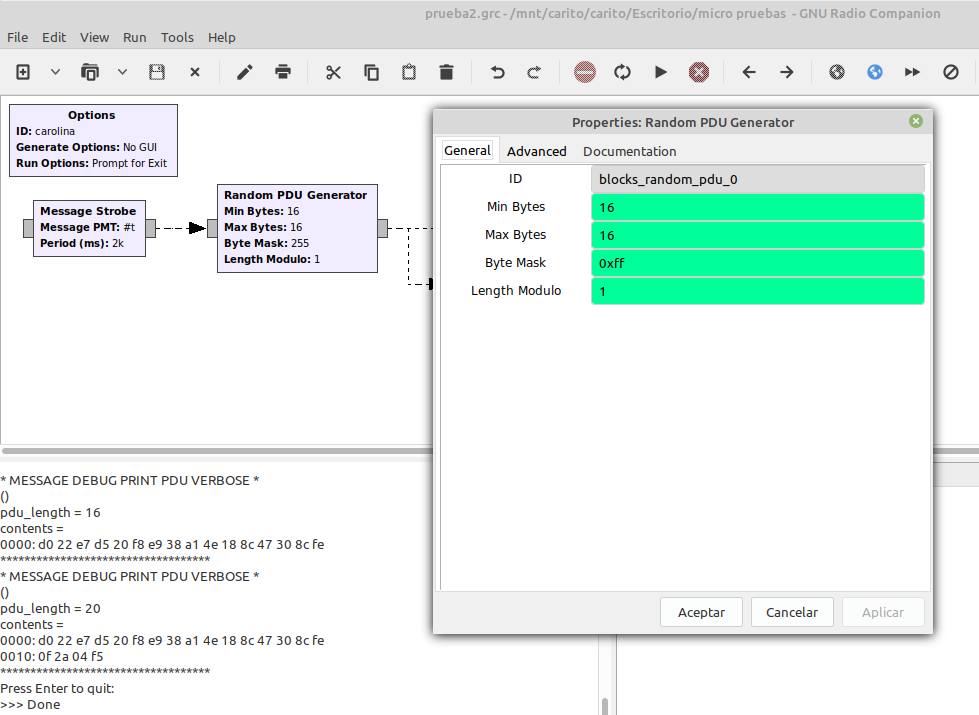
\includegraphics[width=\textwidth]{Modulaciones_digitales/lab25/pdf/bitmap11.pdf}
\end{figure}

\end{frame}
%---------------------------------



\begin{verbatim}

REPUESTA POR CONSOLA 

* MESSAGE DEBUG PRINT PDU VERBOSE *
() pdu length = 20
contents =
0000: d0 22 e7 d5 20 f8 e9 38 a1 4e 18 8c 47 30 8c fe
0010: 0f 2a 04 f5
***********************************
Press Enter to quit:

\end{verbatim}

%---------------------------------
\begin{frame}{EJEMPLO CON MASCARA 0}

\begin{figure}[H]
\centering
\vspace{-3mm}
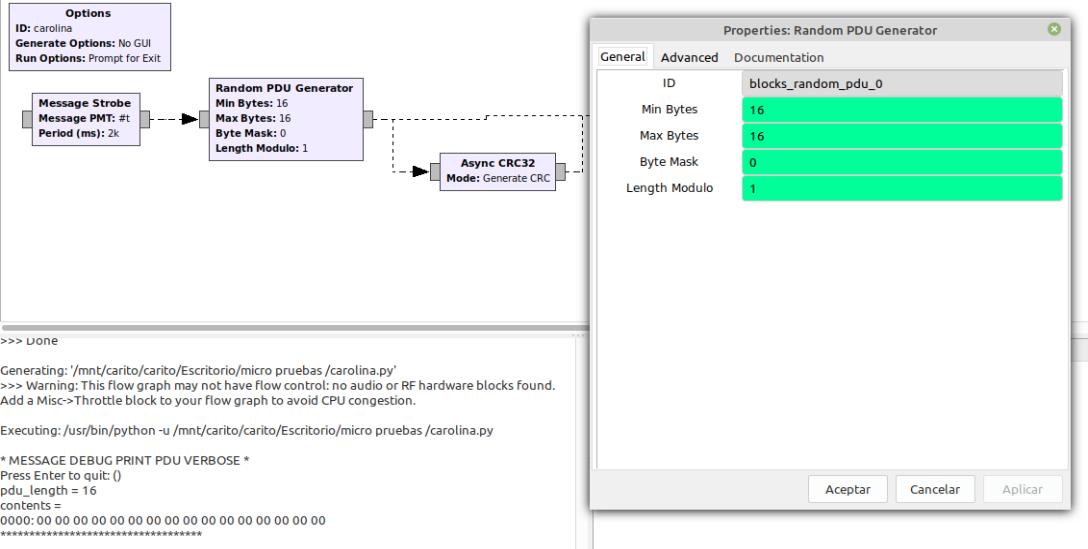
\includegraphics[width=\textwidth]{Modulaciones_digitales/lab25/pdf/bitmap10.pdf}
\end{figure}

\end{frame}
%---------------------------------


\begin{verbatim}

REPUESTA POR CONSOLA 

* MESSAGE DEBUG PRINT PDU VERBOSE *
() pdu length = 20
contents =
0000: 00 00 00 00 00 00 00 00 00 00 00 00 00 00 00 00
0010: 55 4b bb ec
***********************************
Press Enter to quit:

\end{verbatim}


%---------------------------------
